\subsection*{Papaya example}
We will start with an introductory example concerned with papayas. The task in our example is the following: 

\begin{itemize}
  \item \begin{tikzborder}{Boolean classification problem} We want to predict whether a tropical fruit (here a papaya) is tasty or not.\end{tikzborder}
  \item The decision shall be based on observations that we can make from the outside.
  \item \begin{tikzborder}{Supervised learning setting} We get a sample of papayas to try, which we will use as our \textit{training set}.
  \end{tikzborder}
\end{itemize}

\begin{figure}[h]
  \centering
  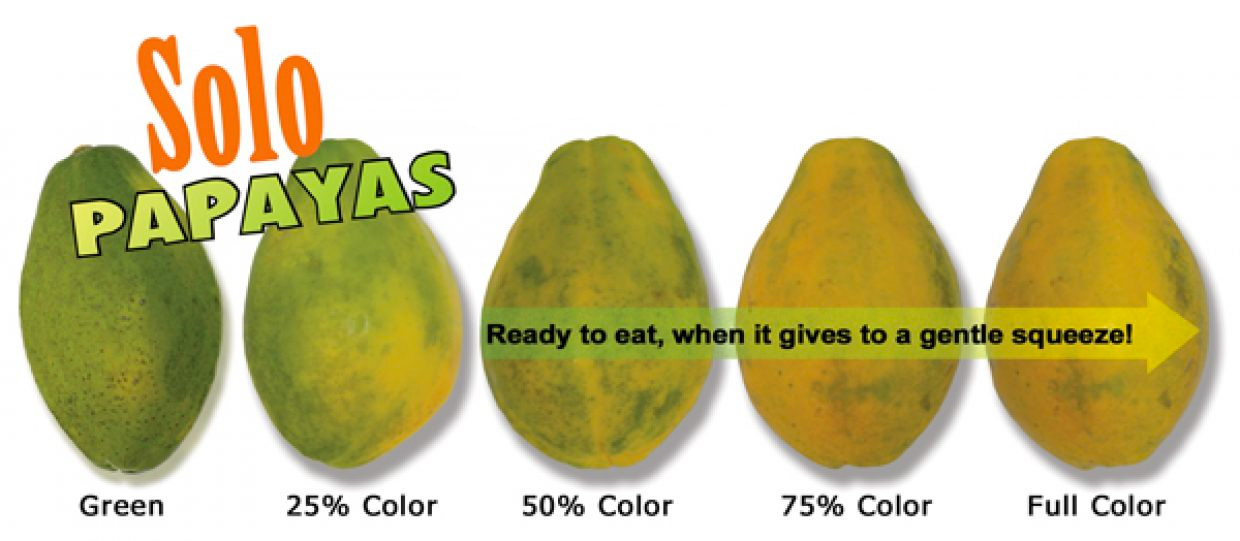
\includegraphics[width=0.6\textwidth]{assets/slf/papayas.jpg} 
  \caption{Papayas with different features}
  \label{fig:1_papaya}
\end{figure}

\begin{tikzborder}{Feature selection} As our first step, we need to select features.\end{tikzborder} Based for example on previous experience with other fruits, we decide to base our decision on these two features of papayas:
\begin{itemize}
  \item Colour, ranging from green through yellow and red to brown
  \item Softness, ranging from hard to mushy
\end{itemize}

When we fill a diagram with our training data to visualize the features and the correct labels as seen in \ref{fig:1_training_set}.

\begin{figure}[h]
  \centering
  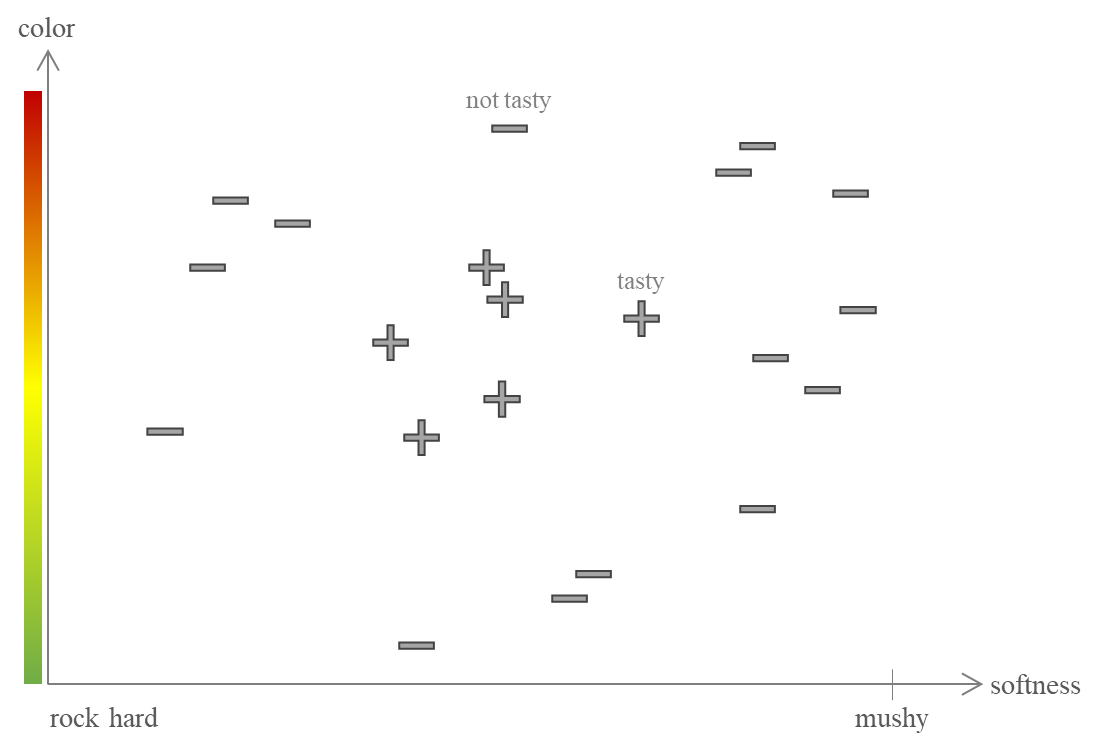
\includegraphics[width=0.7\textwidth]{assets/slf/papaya_testdata__0.png} 
  \caption{Papaya training set}
  \label{fig:1_training_set}
\end{figure}

Next, we select a model and try to fit it optimally with our training data. For that, parameter fitting is applied.
Consider for example a simple \begin{tikzborder}{parametric model}{parametric model}\end{tikzborder} where the features have to lie in a certain range.
\begin{equation*}
  \begin{array}{@{}l@{}}
      \begin{minipage}[b]{0.4\textwidth}
          \begin{itemize}
              \item Color: $[c_{\min}, c_{\max}]$
              \item Softness: $[s_{\min}, s_{\max}]$
          \end{itemize}
      \end{minipage}
  \end{array}
  \left.\begin{array}{@{}c@{}}
      \\
      \\
      \\
  \end{array}\right\}\hspace*{0.2cm}\begin{minipage}{0.6\textwidth}
    4 parameters to be estimated
\end{minipage}
\end{equation*}

\begin{tikzborder}{parameter estimation}Those parameters now need to be estimated in a way, that the resulting hypothesis explains the data best.\end{tikzborder} For that, we choose from a space of all possible \begin{tikzborder}{hypothesis}hypotheses\end{tikzborder}, in this case the set of all axis-parallel rectangles in the color-softness-plane.

\begin{figure}[h]
  \centering
  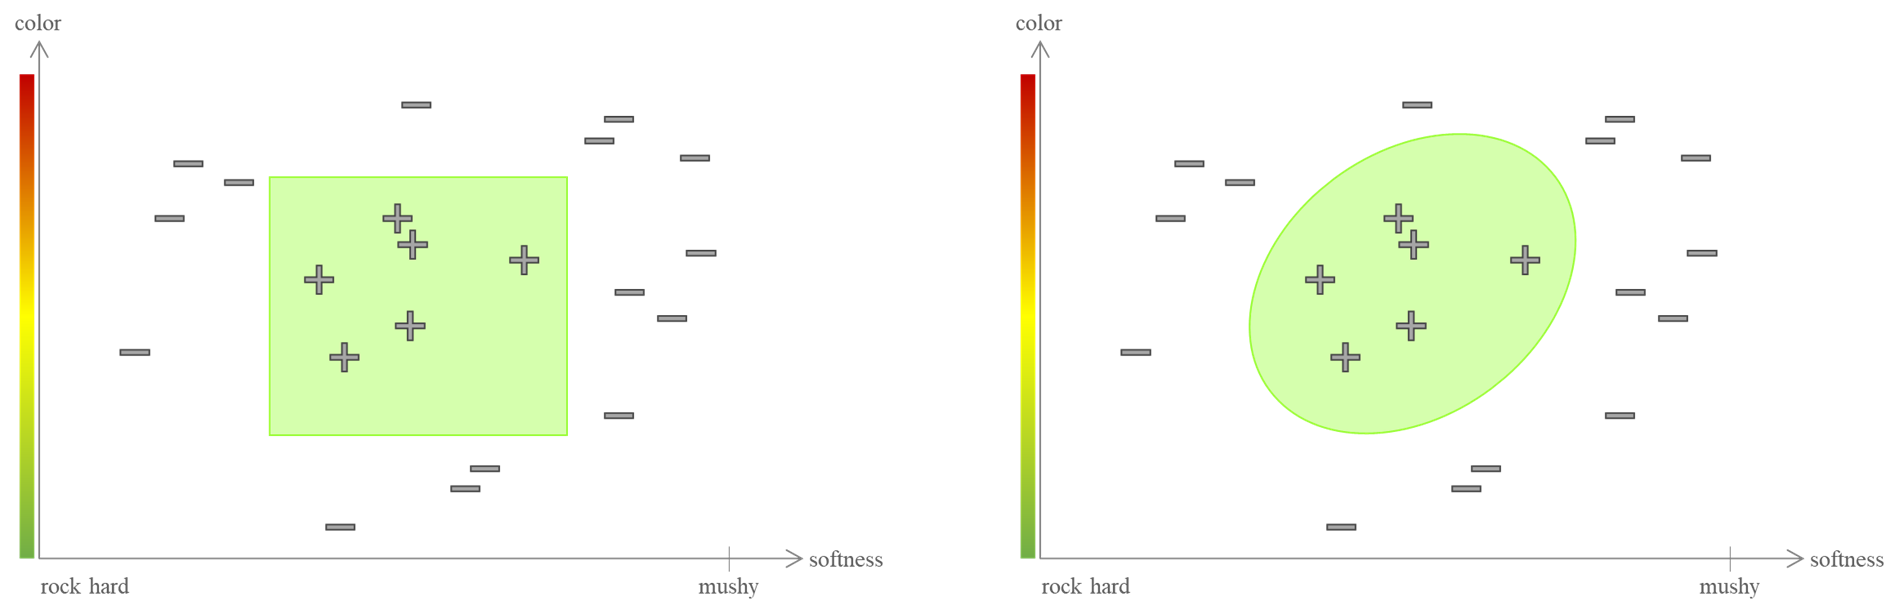
\includegraphics[width=0.9\textwidth]{assets/slf/papaya__1.png} 
  \caption{Papaya hypothesis}
  \label{fig:1_hypothesis}
\end{figure}

Besides the visualized best-fitting hypothesis, one can also see another hypothesis in the image \ref{fig:1_hypothesis}. This one learns the model AND the parameters for this model (assuming there are any) directly. In our example, this learned model looks similar to a Gaussian one.

\begin{tikzborder}{overfitting}A very important problem to keep track of is overfitting, meaning the learned model fits the training data very well, but doesn't generalize to the overall classification in all of the feature space.\end{tikzborder} An extreme example of overfitting would be the following function:
\begin{equation*}
  \text{Function evaluates to }\left\{ \begin{array}{ll}
    1 & \text{ where training examples are positive (tasty)}\\
    0 & \text{ everywhere else}
  \end{array} \right.
\end{equation*}

Back to our rectangular model\footnote{The model where the hypothesis space consists of rectangles in the feature-plane}. This model is extremely simple, maybe even too simple to successfully fulfill our task. Even the feature selection (including the number of features) and the mapping of features to real numbers is questionable. Since it's very likely that not only our selected features determine the tastiness of a papaya alone\footnote{Two papayas with the exact same color and softness might taste differently well}, a more realistic type of model would output a probability that the corresponding papayas are tasty for each point in the plane. The result can look as in image \ref{fig:1_alt_hypo}.

\begin{figure}[h]
  \centering
  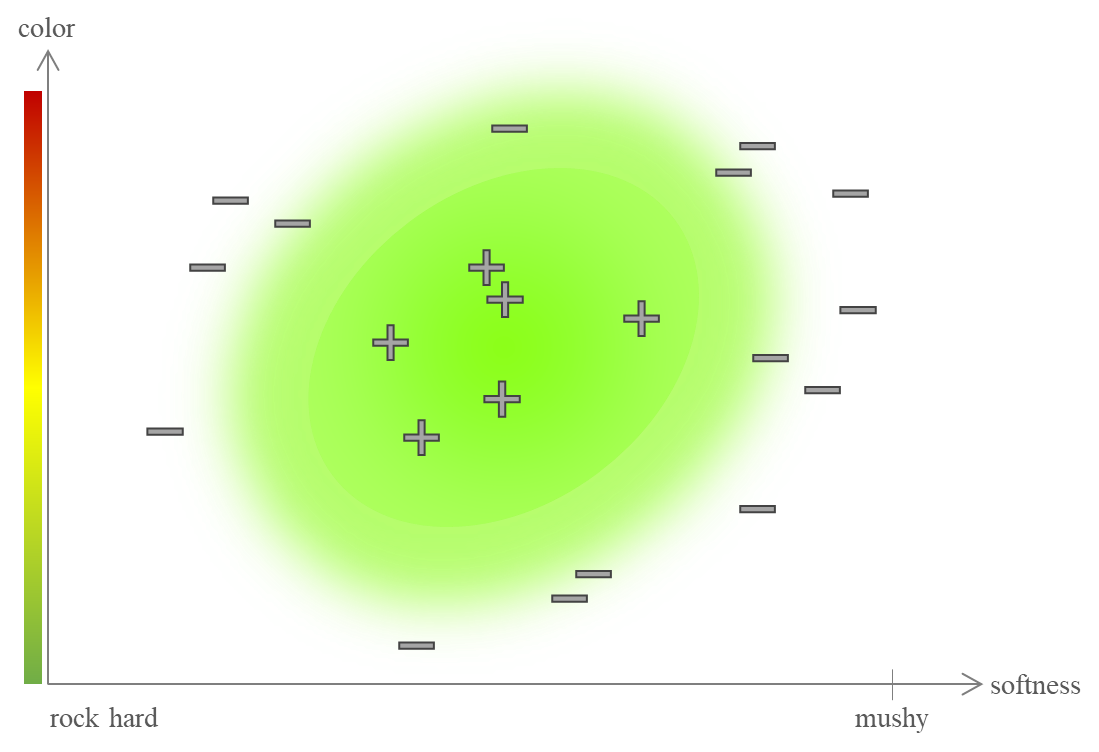
\includegraphics[width=0.45\textwidth]{assets/slf/papaya__2.png} 
  \caption{Papaya probabilistic hypothesis}
  \label{fig:1_alt_hypo}
\end{figure}

